\documentclass{standalone}
\usepackage{tikz}
\usetikzlibrary{decorations.pathmorphing,patterns}
\tikzset{snake it/.style={decorate, decoration=snake},}
\begin{document}
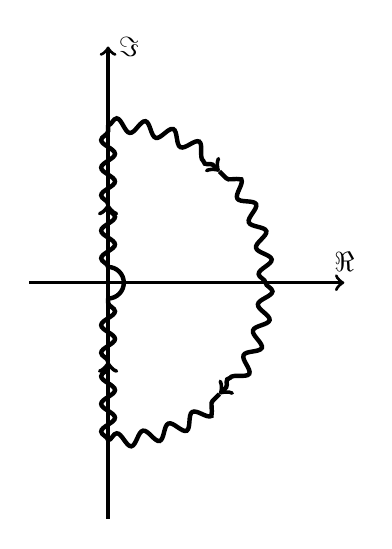
\begin{tikzpicture}[scale=2]
    \draw[->,very thick](-0.5,0)--(1.5,0)node[above]{$\Re$};
    \draw[->,very thick](0,-1.5)--(0,1.5)node[right]{$\Im$};

    \draw[->,snake it, ultra thick](0,-1)--(0,-0.5);
    \draw[-,snake it, ultra thick](0,-0.5)--(0,-0.1);
    \draw[->,snake it, ultra thick](0,0.1)--(0,0.5);
    \draw[-,snake it, ultra thick](0,0.5)--(0,1);

    \draw[-,ultra thick](0,0.1)arc(90:-90:0.1cm);
    
    \draw[->, snake it, ultra thick](0,1)arc(90:45:1cm);
    \draw[-, snake it, ultra thick](1,0)arc(0:45:1cm);       
    \draw[->, snake it, ultra thick](1,0)arc(0:-45:1cm);
    \draw[-, snake it, ultra thick](0,-1)arc(-90:-45:1cm);
\end{tikzpicture}
\end{document}